\chapter{Argumentation Framework} \label{ch:Argumentation Framework}
\section{Definizione di Argumentation Framework}
Come i CSP l'argumentation è un altro metodo che offre l'intelligenza
artificiale per rappresentare la conoscenza e risolvere i problemi. Quello che
andremo a rappresentare sono delle situazioni/dialoghi che vogliamo studiare dal
punto di vista logico.\\
Un argumentation framework (AF) è una coppia (A,R) dove
\begin{itemize}
    \item A è un set di argomentazioni
    \item R $\subseteq$ A $\times$ A è una relazione rappresentante gli "attacchi"
          ("sconfitte")
\end{itemize}
\begin{center}
    $F(\{a,b,c,d,e\}, \{(a,b),(c,b),(c,d),(d,c),(d,e),(e,e)\})$
\end{center}
\begin{figure}[H]
    \centering
    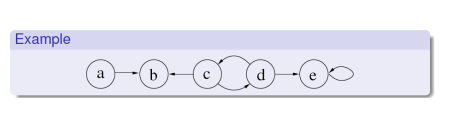
\includegraphics[width=12cm, keepaspectratio]{img/Cap6/arg1.png}
    \caption{Argumentation framework}
\end{figure}

Si ha un attacco quando si ha un'espressione logica (frase, dato...) che è in
contraddizione con un'altra. Gli attacchi possono essere anche pesati, essi
possono dipendere anche da chi ha detto quella frase.

\begin{figure}[H]
    \centering
    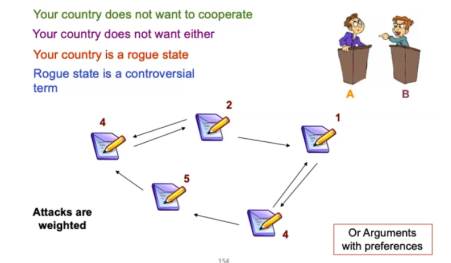
\includegraphics[width=12cm, keepaspectratio]{img/Cap6/arg2.png}
    \caption{Esempio di argumentation framework}
\end{figure}
Ci possono essere anche casi in cui è noto chi dice l'argomento e altri in cui
non lo è. Per quest'ultima vogliamo selezionare gli argomenti che sono più
validi rispetto agli altri, ad esempio in Figura 6.2 il 4 e il 2 sembrano buoni
argomenti perché attaccano gli altri e contrattaccano nel caso siano attaccati.
Lo scopo è di definire dei criteri per trovare gli argomenti più forti, validi
(che stanno "in piedi da soli"), in modo da selezione i conflitti che riescono a
sopportare gli attacchi dall'esterno.

\begin{figure}[H]
    \centering
    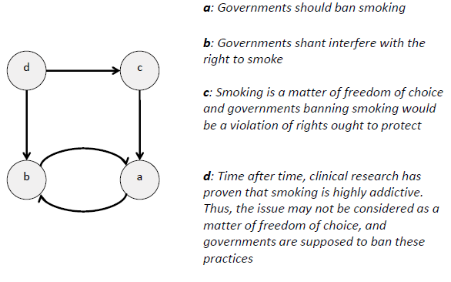
\includegraphics[width=12cm, keepaspectratio]{img/Cap6/arg3.png}
    \caption{Altro esempio di argumentation framework}
\end{figure}

Dobbiamo trovare gli argomenti che "stanno bene insieme", la prima nozione di
questo tipo è un insieme di argomenti senza conflitti.

\section{Tipologie di semantiche}
Esistono principalmente tre tipologie di semantiche basate sulla metodologia
con la quale vengono calcolate.
\begin{enumerate}
    \item \textbf{Estensione:} Andiamo a guardare dei sottoinsieme di
          argomenti (tutte quelle viste precedentemente)
    \item \textbf{Labeling:} Il labeling è una funzione che assegna delle
          etichette (colori) ad ogni argomento in modo tale da distinguere gli
          argomenti accettati dai restanti.
    \item \textbf{Ranking:} Restituisce un ordimento sugli argomenti. Dice
          quindi "l'argomento a è migliore di b". Questo sistema è più raffinato.
\end{enumerate}

\section{Extension-Based Semantics}
Il task principale che viene svolto sugli argumentation framework è il computo
della semantica, cioè si selezionano dei criteri con i quali si vanno a
scegliere dei sottoinsiemi di argomenti che condividono una qualche proprietà
particolare. Di seguito una breve descrizione:
\begin{itemize}
    \item \textbf{Conflict Free}: Argomenti che non si attaccano.
    \item \textbf{Admissible}: Richiede la nozione di difesa, cioè un
          contrattacco che un argomento fa ad un altro argomento che è attaccato.
    \item \textbf{Complete}: Deve essere admissible, se un argomento è
          difeso questo è per forza dentro l'estensione. Nell'esempio sopra a era
          l'unico argomento che era sempre difeso (non veniva attaccato da
          nessuno) quindi l'insieme complete sono tutti gli argomenti che hanno
          dentro a.
    \item \textbf{Preferred}: Si ottiene per inclusione insiemistica, cerco
          le admissible più grandi. tra \{a\},\{c\},\{d\},\{a, c\},\{a, d\} dato
          che voglio la più grande, la singola {a} non potrà essere preferred,
          perché si trova dentro \{a, c\},\{a, d\} che sono più grandi.
    \item \textbf{Grounded}: Set più piccolo tra tutte le complete.
    \item \textbf{Stable}: Seleziono un insieme di argomenti che è conflict
          free e che attacca tutti gli altri
\end{itemize}

La prima che vediamo è quella degli insiemi Conflict Free, cioè
quegli insiemi che tra loro non hanno conflitti.

\subsection{Estensioni Conflict-Free}
Dato un Augmentation Framework F = (A, R), l'insieme S $\subseteq$ A è
conflict-free se, per ogni (a, b) $\in$ S, si ha che (a, b) $\notin$ R. (Per
ogni coppia di elementi in S non è presente una relazione d'attacco tra questi
elementi).

\begin{figure}[H]
    \centering
    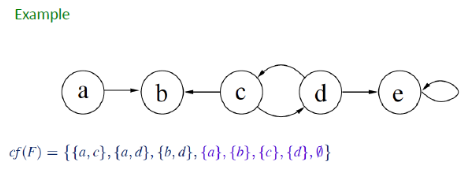
\includegraphics[width=12cm, keepaspectratio]{img/Cap6/cf.png}
    \caption{Esempio insieme conflict-free.}
\end{figure}

In questo caso andiamo a scegliere come coppie gli argomenti che non sono in
conflitto (quindi che non si attaccano) fra di loro, ($\{a,c\},\{a,d\}$ ma non $\{a,b\}$),
e anche i singoli argomenti tranne e poiché esso si contraddice da solo visto
che ha un cappio.

\paragraph{Importante:} per il calcolo: inizio con inserire
\textbf{l'insieme vuoto}, poi i \textbf{singoli} argomenti che non si
auto-attaccano, poi \textbf{le coppie, terne, quadruple...}

\subsection{Estensioni Admissible}
Dato un Augmentation Framework F = (A, R), l'insieme S $\subseteq$ A è
ammissibile se:
\begin{itemize}
    \item S è \textbf{conflict free;}
    \item Ogni a $\in$ S è \textbf{difeso} da S (cioè ogni elemento che
          appartiene all'insieme è difeso dagli elementi dell'insieme stesso). Un
          elemento a $\in$ A è difeso da S se, per ogni b $\in$ A con (b, a) $\in$ R,
          esiste un c $\in$ S tale per cui (c, b) $\in$ R (a è difeso da S se per ogni
          b che attacca quell'elemento a esiste un altro elemento sempre dentro S che
          contrattacca l'attacco di b verso a).
\end{itemize}

\begin{figure}[H]
    \centering
    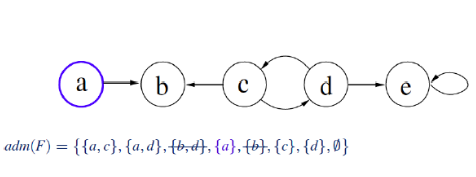
\includegraphics[width=12cm, keepaspectratio]{img/Cap6/ammissibile.png}
    \caption{Esempio insieme Ammissibile.}
\end{figure}

Non è necessario che sia lo stesso argomento a difendersi da altri attacchi, ad
esempio in questo caso, supponendo che non ci sia a, b è attaccato da c ma se
prendo d lui oltre che difendere se stesso da c (poiché attaccato) difende anche
b. Guardando la definizione di difesa, un argomento a è difeso da un argomento
b, (b, a) $\in$ R, nel momento in cui esiste un argomento c tale che c attacca
b, (c, b) $\in$ R. Il sottoinsieme \{b,d\} non viene scelto poiché d è attaccato
da c ma a si difende a sua volta contrattaccando, mentre b è attaccato sia da a
che c, nel primo caso nessuno lo difende nel secondo d difende b perché attacca
c.
\begin{itemize}
    \item l'insieme $\emptyset$ (vuoto) è \textbf{ammissibile}? Si, nessuno lo attacca.
    \item l'insieme $\emptyset$ (vuoto) è \textbf{Conflict Free}? Si.
\end{itemize}

\subsection{Estensioni Complete (Tutti Difesi)}
Dato un Augmentation Framework F = (A, R), l'insieme S $\subseteq$ A è completo
se:
\begin{itemize}
    \item S è ammissibile;
    \item Ogni a $\in$ A admissible difeso da S è contenuto in S. Un elemento a $\in$ A è
          difeso da S se, per ogni b $\in$ A con (b, a) $\in$ R, esiste un c $\in$ S
          tale per cui (c, b) $\in$ R.
\end{itemize}
\begin{figure}[htp]
    \centering
    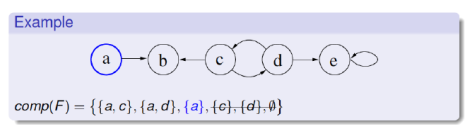
\includegraphics[width=12cm, keepaspectratio]{img/Cap6/completo.png}
    \caption{Esempio insieme Completo.}
\end{figure}
Quindi un insieme complete contiene tutti gli insiemi ammissibili e anche tutti
gli argomenti che sono difesi.\\
L'insieme $\emptyset$ (vuoto) è \textbf{Completo}? Va messo
soltanto quando tutti gli argomenti sono attaccati e quindi quando \textbf{non}
c'è un qualche argomento che è sempre difeso.\\
Infatti sopra non va messo
perché a è sempre difeso. a è sempre difeso da tutti perché non è attaccato da
nessuno, quindi nel calcolo dei difensori va sempre messo dentro.
\begin{enumerate}
    \item \{a, c\} è \textbf{completo?} Si!
          \begin{itemize}
              \item a chi difende? attacca b quindi difenderebbe tutti quelli
                    attaccati da b, ma b non attacca nessuno quindi a difende solo se
                    stesso.
              \item c chi difende? tutti quelli attaccati da b quindi nessuno e
                    tutti quelli attaccati da d quindi c.
          \end{itemize}
          \textbf{L'insieme dei difensori è a, c, che sta dentro S=\{a, c\},
              quindi è completo.}
    \item \{a, d\} è \textbf{completo?}
          \begin{itemize}
              \item a chi difende? attacca b quindi difenderebbe tutti quelli
                    attaccati da b, ma b non attacca nessuno quindi a difende solo se
                    stesso.
              \item d chi difende? se stesso, perché viene attaccato da c ma si
                    difende da solo con un contrattacco.
          \end{itemize}
          L'insieme dei difensori è \{a, d\} che sta dentro S quindi anche
          questo è completo. \\\{a\} è \textbf{completo?} Può stare da solo
          perché non viene attaccato da nessuno, quindi è \textbf{come se
              venisse difeso da tutti quanti}, e lui non difende nessuno, poiché b
          non attacca nessuno. \\Quindi se un argomento non attaccato da nessuno
          ne attacca un altro che a sua volta non attacca nessuno allora
          quell'elemento è complete e può stare da solo. \\\{c\} è
          \textbf{completo?} Difensori: \{a, c\} che non è incluso in c quindi
          No. \\\{d\} è \textbf{completo?} Difensori: \{a, d\} quindi No. L'idea
          degli insiemi complete è che se un insieme difende qualcosa, quel
          qualcosa ”deve essere messo dentro” e \textbf{deve rimanere
              ammissibile.}

          \vspace{0.8cm}

          La differenza quindi è che nell'insieme ammissibile vuol dire che mi
          difendo, complete vuol dire che dentro ci sono tutti quelli difesi.
\end{enumerate}
\
\subsection{Estensioni Grounded (Minimale)}
F = (A, R), l'insieme S $\subseteq$ A è grounded se:
\begin{itemize}
    \item S è \textbf{completo};
    \item Per ogni sotto insieme T $\subseteq$ A completo in F si ha che T
          $\subsetneq$ S
\end{itemize}
Quindi un insieme completo è grounded se è il \textbf{più piccolo dei complete},
ovvero se \textbf{non} esiste un sottoinsieme T complete che è più piccolo di
lui. Si calcola tramite \textbf{l'intersezione} delle complete. \textbf{N.B}
L'insieme grounded è sempre \textbf{UNICO}, cioè composto da un solo elemento.
\begin{figure}[htp]
    \centering
    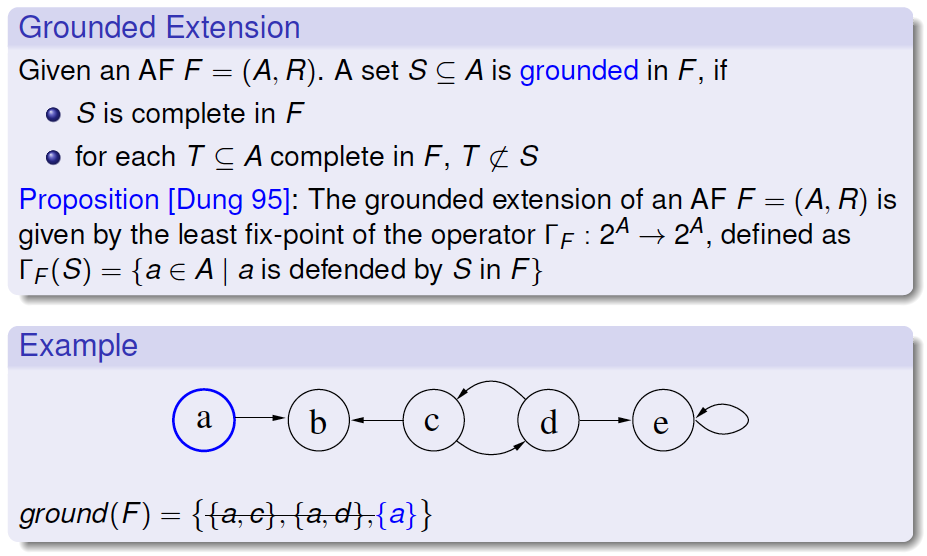
\includegraphics[width=12cm, keepaspectratio]{img/Cap6/grounded.png}
    \caption{Esempio Grounded}
\end{figure}
\\a, c è \textbf{grounded}? i suoi sottoinsiemi singoli sono a e c, questi sono
completi? \\no, perché a lo è ma non c quindi non è grounded. \\a, d è
\textbf{grounded}? i suoi sottoinsiemi singoli sono a e d, questi sono completi?
\\no, perché a lo è ma non d quindi non è grounded. \\a è \textbf{grounded}? Si,
i suoi sottoinsiemi singoli sono a ed è completo.

\vspace{0.8cm}

\textbf{N.B} L'insieme grounded è dato anche dall'intersezione di tutti gli
insiemi completi, infatti sopra se intersechiamo quei 3 insiemi completi l'unica
cosa che viene fuori era a che infatti è l'unico insieme grounded.

\subsection{Estensioni Preferred (Massimale)}
Dato un Augmentation Framework F = (A, R), l'insieme S $\subseteq$ A è preferred
se:
\begin{itemize}
    \item S è ammissibile;
    \item Per ogni sotto insieme T $\subseteq$ A ammissibile in F , si ha che S
          $\subsetneq$ T (cioè se nessuno degli ammissibili S è più grande di T).
\end{itemize}
\begin{figure}[htp]
    \centering
    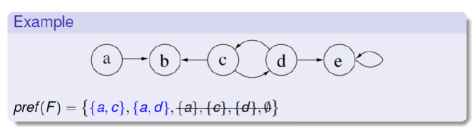
\includegraphics[width=12cm, keepaspectratio]{img/Cap6/prefered.png}
    \caption{Esempio Preferred}
\end{figure}
Si ottiene per inclusione insiemistica, \textbf{Le più grandi delle admissible}.
(a) da solo è contenuto in (a,c) che è più grande quindi sicuramente non sarà
preferred, stessa cosa per (d). (c) stessa cosa per (a,c). \\Al contrario di
grounded dove si andava a scegliere l'insieme con l'elemento in comune con gli
altri insieme, in questo caso si va a scegliere tra gli insiemi ammissibili
quelli che sono più grandi. Da notare che si sceglie tra gli insiemi ammissibili
ma si può dimostrare che si può scegliere da quelli complete.

\subsection{Estensioni Stable}
Dato un AF, F=(A,R). Un insieme S $\subseteq$ A è stabile in F, se
\begin{itemize}
    \item S è \textbf{conflict-free} in F
    \item per ogni a $\in$ A / S, esiste una b $\in$ S, tale che (b, a) $\in$ R.
\end{itemize}
\begin{figure}[htp]
    \centering
    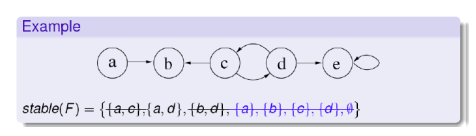
\includegraphics[width=12cm, keepaspectratio]{img/Cap6/stable.png}
    \caption{Esempio Stable}
\end{figure}
Per ogni elemento fuori da S esiste un elemento di S che lo attacca. Questo
significa che gli insiemi stable sono gli insiemi conflict-free che attaccano
tutti gli altri, ovvero che tutti gli elementi che stanno fuori dall'insieme
esaminato sono attaccati.\\
In questo caso si sceglie l'insieme i quali elementi attaccano tutti gli
elementi fuori dall'insieme conflict-free, ad esempio \{a,c\} non si prende
perché a attacca b e c attacca d e b ma nessuno dei due attacca e. Mentre
nell'insieme \{a,d\} a attacca b e d attacca sia c che e. Esiste anche una
semantica semi-stabile la quale nel caso cui esista un insieme stabile allora
essa coincide con quest'ultimo ma quando non c'è la stabile allora sceglie tra
gli insieme preferred quelli che ne attaccano di più tra gli insiemi fuori a
quest'ultimo. L'obiettivo della semantica stabile è di avere cardinalità più
grande possibile e di attaccare tutti gli insiemi fuori.

\vspace{0.5cm}

\noindent a, c \textbf{non è stabile} perché è si ammissibile (b che sta fuori è
attaccato e ok), d sta fuori ed è attaccato, ma e non lo attacca ne a ne c
quindi questo insieme non può essere stabile. \\a, d \textbf{è stabile} perché a
attacca b e d attacca c, e quindi tutti gli elementi fuori dall'insieme sono
attaccati. \\La semantica stabile è la più forte di tutte le Estensioni, perché
sono le posizioni più forti in un dialogo, sono la scelta migliore quando
utilizzo AF come decision making. Il problema delle Estensioni stabili è che non
sempre esistono.

\section{Labeling-Based Semantics}
Il Labeling è una funzione che assegna delle etichette rappresentate come
colori ad ogni argomento. Le etichette sono di tre tipi:
\begin{enumerate}
    \item \textbf{Verdi:} Corrispondono ad argomenti IN, cioè sono ”dentro”
          l'insieme di argomenti accettati.
    \item \textbf{Rosse:} Corrispondono ad argomenti OUT, cioè sono ”fuori”
          dall'insieme di argomenti accettati.
    \item \textbf{Gialle:} ”Undecided” e sono fuori dagli insiemi
          direttamente accettati(verdi) ma non sono direttamente Rejected (rossi),
          ovvero non ho una motivazione esplicita per non accettare quel nodo,
          quindi sono una via di mezzo.
\end{enumerate}
Qualsiasi assegnamento di colori è un labeling (posso colorare tutti i nodi
di verde e apposto), però chiaramente non rispetterà le semantiche che
adesso introdurremo. Le semantiche basate su labeling corrispondono
esattamente alle semantiche basate su Estensioni, ed infatti possiamo
calcolare le stesse cose.

\subsection{Labeling Conflict-Free}
Per ogni argomento $a \in A$ si ha che:
\begin{itemize}
    \item $a$ è \textbf{IN} se non ha altri attaccanti IN.
    \item $a$ è \textbf{OUT} se è attaccato da almeno un argomento IN.
\end{itemize}
\begin{figure}[H]
    \centering
    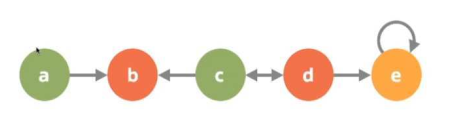
\includegraphics[width=12cm, keepaspectratio]{img/Cap7/CF.png}
    \caption{Esempio di Conflict-Free Labeling.}
\end{figure}
\begin{itemize}
    \item $a$ è verde perché non ha nessun altro argomento verde che lo
          attacca.
    \item $c$ è verde per lo stesso motivo
    \item $b$ e $d$ sono rossi perché c'è almeno un argomento verde che li
          attacca.
    \item $e$ è attaccato da un argomento rosso, ma le regole non
          specificano il colore in questo caso, quindi l'argomento resta fuori sia
          dalla colorazione IN che OUT. Per esprimere questa incertezza utilizzo
          la label gialla.
\end{itemize}
\textbf{Domanda: } Questo labeling sotto è conflict free? (cioè soddisfa le
regole scritte sopra?)
\begin{figure}[H]
    \centering
    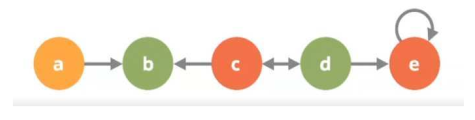
\includegraphics[width=12cm, keepaspectratio]{img/Cap7/CF2.png}
    \caption{Conflict free label}
\end{figure}
\begin{center}
    \textbf{Si, nessuna regola viene violata.}
\end{center}

\textbf{Domanda: } Questo labeling sotto è conflict free?
\begin{figure}[H]
    \centering
    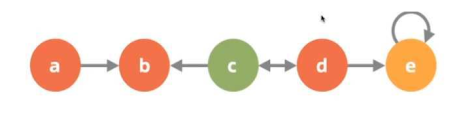
\includegraphics[width=12cm, keepaspectratio]{img/Cap7/CF3.png}
    \caption{No conflict free label}
\end{figure}
\begin{center}
    \textbf{No! perché a è rosso ma non ha un argomento verde che lo attacca.}
\end{center}

\subsection{Labeling Admissible}
Per ogni argomento $a \in A$ si ha che:
\begin{itemize}
    \item $a$ è \textbf{IN} se tutti i suoi attaccanti sono OUT.
    \item $a$ è \textbf{OUT} se è attaccato da almeno un argomento IN.
\end{itemize}
In questo caso c'è la nozione di Difesa, ovvero che un argomento è accettato
(è IN) solamente se \textbf{tutti} i suoi attaccanti sono sconfitti (OUT)
\begin{figure}[H]
    \centering
    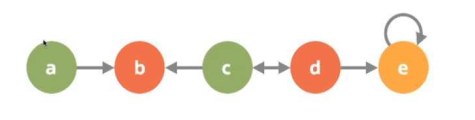
\includegraphics[width=12cm, keepaspectratio]{img/Cap7/LA.png}
    \caption{Esempio Labeling Admissible}
\end{figure}

Questo labeling è admissible, ad esempio c è accettato perché d che lo
attacca è sconfitto, cioè OUT.
\begin{figure}[H]
    \centering
    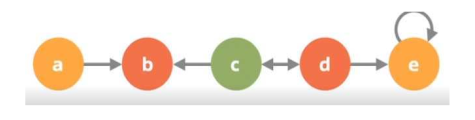
\includegraphics[width=12cm, keepaspectratio]{img/Cap7/LA2.png}
    \caption{Esempio2 Labeling Admissible}
\end{figure}
Questo esempio è comunque admissible, perché non ho obblighi sull'argomento
a, posso etichettarlo di Verde e la regola sarebbe soddisfatta, ma non
avendo attaccanti posso etichettarlo sia giallo che verde e non violo
nessuna regola.

\paragraph{Differenza:} la differenza tra Admissible e Complete
è che A in complete deve essere per forza verde mentre qui può essere anche
giallo.

\subsection{Labeling Complete}
Per ogni argomento $a \in A$ si ha che:
\begin{itemize}
    \item  $a$ è \textbf{IN} \textit{se e solo se} tutti i suoi attaccanti
          sono etichettati come OUT o quell'argomento non ha attaccanti.
    \item $a$ è \textbf{OUT} \textit{se e solo se} è attaccato da almeno un
          argomento IN.
\end{itemize}
\textbf{Domanda: } Questo labeling è complete?
\begin{figure}[H]
    \centering
    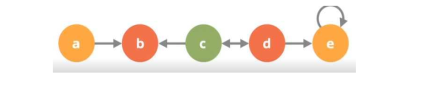
\includegraphics[width=12cm, keepaspectratio]{img/Cap7/LC.png}
    \caption{Esempio Labeling NON COMPLETE}
\end{figure}
No, perché l'argomento a è etichettato di giallo, ma la prima regola mi
dice che un argomento è etichettato di verde quando tutti i suoi attaccanti
sono etichettati di rosso, ma ho un se e solo se, devo leggerlo anche dalla
parte opposta, ovvero:

\vspace{0.3cm}
\noindent É IN se ha tutti attaccanti etichettati OUT, ma dato che a non ha
attaccanti deve per forza essere verde, cosi come d.

\vspace{0.3cm}

\noindent \textbf{La differenza} con l'admissible è proprio quel ”se e solo
se”. L'admissible ci permette di ignorare degli elementi che potrebbero
essere accettati (infatti posso sia etichettarlo verde o giallo a prima), ma
questo non accade nella complete, cioè se tutti gli argomenti che mi
attaccano sono out (e questo accade anche quando nessun argomento mi
attacca) allora devo essere per forza verde. \\
Il labeling complete dell'esempio sarebbe:
\begin{figure}[H]
    \centering
    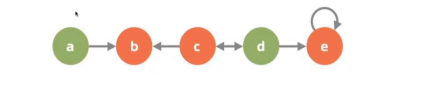
\includegraphics[width=12cm, keepaspectratio]{img/Cap7/LC2.png}
    \caption{Esempio Labeling COMPLETE}
\end{figure}

\subsection{Labeling Grounded (Minimale)}
Il labeling deve essere:
\begin{itemize}
    \item \textbf{Completo}
    \item L'insieme degli argomenti \textbf{IN} deve essere
          \textbf{Minimale} tra tutte le labeling complete.
\end{itemize}
\subsection{Labeling Preferred (Massimale)}
\begin{itemize}
    \item \textbf{Completo}
    \item L'insieme degli argomenti \textbf{IN} deve essere
          \textbf{Massimale} tra tutte le labeling complete.
\end{itemize}
\begin{figure}[H]
    \centering
    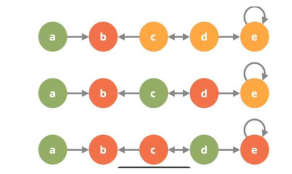
\includegraphics[width=12cm, keepaspectratio]{img/Cap7/GR.png}
\end{figure}
Di queste:
\begin{enumerate}
    \item \textbf{Grounded} perché solo l'argomento $a$ è IN. L'argomento
          $a$ dovrà essere in qualsiasi estensione IN, proprio perché non essendo
          attaccato la regola dice che deve per forza essere IN.
    \item \textbf{Preferred} questa è sicuramente Admissible.
    \item \textbf{Preferred}: $a$, $d$ è massima rispetto l'inclusione.
\end{enumerate}

\section{Ranking-Based Semantics}
Un ranking è un ordinamento parziale o totale di un insieme di argomenti.
Quello che ottengo da una semantica di ranking è un vero e proprio
ordinamento, cioè una cosa del tipo:
\begin{center}
    $a > d > c > e >b$
\end{center}
e non un insieme come lo era fino ad adesso. Quindi potremo dire quando un
argomento è ”migliore” rispetto ad un altro. Possiamo avere:
\begin{itemize}
    \item Ordinamento \textbf{quantitativo:} Consiste nell'assegnare prima
          dei punteggi agli argomenti come "a vale 5, b vale 7" quindi concludo
          che b è migliore.
    \item Ordinamento \textbf{qualitativo}: "Seguendo questo ordinamento
          l'argomento a è migliore dell'argomento d.
\end{itemize}
\begin{center}
    Metodi visti
\end{center}
\begin{enumerate}
    \item Categorizer
    \item Graded Defense: $a_1 \in d^1_{1} (X_1)$
    \item Shapely Value
\end{enumerate}
\subsection{Ordinamento quantitativo}
\subsubsection{Categorizer}
Ordina gli argomenti utilizzando la seguente funzione:
\begin{enumerate}
    \item Per ogni argomento guarda il numero degli attacchi che riceve.
    \item Utilizza questo valore per assegnare un ranking a tale argomento.
\end{enumerate}
\textbf{In altre parole abbiamo:} Se sono attaccato da argomenti deboli
allora sono un argomento forte; se sono attaccato da argomenti forti sono un
argomento debole.
\begin{figure}[htp]
    \centering
    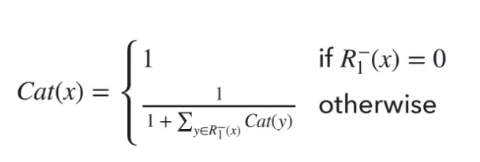
\includegraphics[width=10cm, keepaspectratio]{img/Cap8/quantitativo1.png}
    \caption{Funzione categorizer.}
\end{figure}
Se un argomento non ha attaccanti $R^-1$ $(x) = 0$ allora il valore è 1
sennò è dato 1 dalla formula $\frac{1}{1+\sum_{y\in R^-1_(x)} Cat(y)}$, questo
significa che se ho attaccanti forti allora l'argomento x è debole

\begin{figure}[htp]
    \centering
    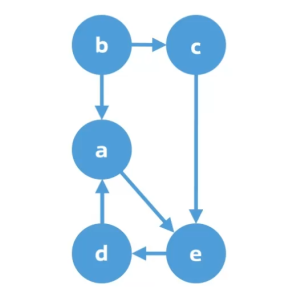
\includegraphics[width=5cm, keepaspectratio]{img/Cap8/quantitativo2.png}
    \caption{Esempio categorizer.}
\end{figure}
\noindent \textbf{Spiegazione: } Si parte sempre dagli iniziatori del grafo,
cioè gli argomenti non attaccati.
\begin{itemize}
    \item $b:$ Ha valore 1 perché la frase: ”non ha attaccanti” si traduce
          in $R^-_1(x) = 0$ quindi va nella prima opzione della funzione, si
          arresta subito e torna 1.
    \item $c:$ Non vale la prima opzione perché è attaccato da b, quindi
          seconda opzione e calcolo 1 + la sommatoria dei valori dei suoi
          attaccanti cioè 1 solamente b. Quindi verrebbe $\frac{1}{1+1}$ = 0.5
\end{itemize}
In questo caso Cat(b)=1 perché non ha attaccanti e Cat(c)=0.5 perché è
attaccato da b con punteggio 1. Mentre Cat(a)=0.38, Cat(d) =0.65 e Cat(e) =
0.53.

\vspace{0.3cm}

Si continua cosi per tutti gli argomenti. Infine si ordinano i risultati e
si ottiene un ordinamento sui rispettivi argomenti:
\begin{center}
    $b>d>e>c>a$
\end{center}
Quindi $b$ è preferito tramite la funzione $cat$ a $d$ e cosi via.
\subsection{Ordinamento Qualitativo}
I principi sono simili a quello precedente:
\begin{itemize}
    \item più è grande il numero degli attaccanti su un argomento b, più è
          debole il livello di giustificazione di b
    \item più è grande il numero di argomenti che difendono a, più è forte
          il livello di giustificazione di a.
\end{itemize}
\subsubsection{Graded Defense, Dung's Theory}
In questo caso andiamo a definire una relazione di preferenza tra le coppie
dei possibili argomenti \textbf{(non si assegnano punteggi)}. I principi che
utilizzeremo sono due:
\begin{enumerate}
    \item Più attaccanti un argomento ha, peggiore è quell'argomento.
    \item Più argomenti sono in mia difesa, più un argomento è forte.

\end{enumerate}
Suddivido gli argomenti con la \textbf{funzione}: $d^m_n$ (X) che
rappresenta tutti quegli argomenti che \textbf{non} hanno almeno $m$
attaccanti che a loro volta \textbf{non} sono contrattaccati da almeno $n$
argomenti.

\vspace{0.3cm}

\textbf{Esempio}

\begin{figure}[htp]
    \centering
    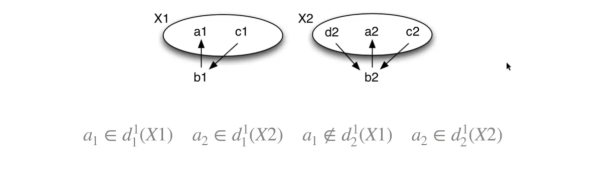
\includegraphics[width=13cm, keepaspectratio]{img/Cap8/defense.png}
    \caption{Esempio graded defense.}
\end{figure}
$a_1$ ha un attaccante ed un difensore, quindi appartiene. a1 ha si un
attaccante, ma non ha due difensori, quindi non appartiene.

\begin{itemize}
    \item $a_1 \in d^1_1$ (X1): non c'è almeno 1 attaccante che non sia
          attaccato a sua volta da almeno 1 argomento. Questo vuol dire che c'è
          almeno un argomento che è contrattaccato da almeno un altro argomento.
          Infatti a1 è attaccato da b1 che è a sua volta attaccato da c1 .
    \item $a_2 \in d^1_1$ (X2): non c'è un argomento che attacca a2 che a
          sua volta non sia contrattaccato da almeno un altro argomento, ma
          addirittura $c_i$ sono due argomenti (che sarebbero $d_2$ , $c_2$ ) che
          contrattaccano l'attaccante di $a_2$ (che sarebbe $b_2$ ), quindi
          diciamo anche che $a_2 \in d^2_1$ (X2). (Esiste un attaccante di $a_1$
          ma non esistono due difensori di $a_1$).
\end{itemize}
\begin{center}
    $a_2 \in d^1_2$ (X2)
\end{center}
Va letto come: Non esiste un argomento (quindi prima l'esponente) che non
sia contrattaccato da almeno 2 argomenti (quindi poi il pedice). Gli
attaccanti li leggo ad apice, i difensori (cioè chi attacca il mio
attaccante) li leggo a pedice. Il dilemma che ci troviamo davanti è:
\begin{center}
    É meglio essere poco attaccati (cioè apice basso) o è meglio avere tanti
    difensori (pedice alto?)
\end{center}
In formule sarebbe: appartenere a $d^3_1$ è meglio o peggio di appartenere a
$d^1_3?$

\paragraph{Formula}
\begin{center}
    $d^m_n$ è meglio di $d^s_t$ $\Leftarrow \Rightarrow$ m $<=$ s AND t $<=$
    n
\end{center}
Cioè un argomento non attaccato da almeno m argomenti che non siano
contrattaccati da almeno n difensori è meglio della stessa cosa con s e t se
e solo se il primo argomento ha sia \textbf{meno attaccanti}, cioè m $<=$ s
che \textbf{più difensori} t $<=$ n. \\Altri esempi: leggere solamente
l'appartenenza.
\begin{figure}[H]
    \centering
    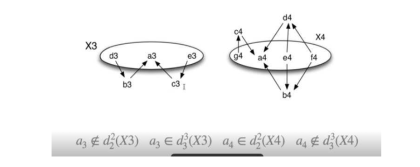
\includegraphics[width=12cm, keepaspectratio]{img/Cap8/defense2.png}
\end{figure}

\paragraph{Applicazione della Graded Semantics ad un grafo}
\begin{figure}[H]
    \centering
    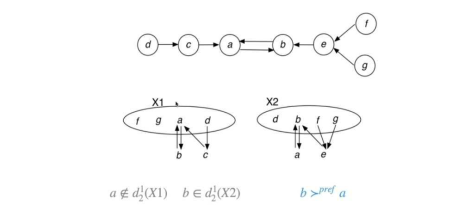
\includegraphics[width=12cm, keepaspectratio]{img/Cap8/GdefnseGrafo.png}
\end{figure}
\textbf{Ci domandiamo:} è vero che a $\in$ $d^1_2$ (X1)? \\Cioè è
vero che a non è attaccato da almeno un argomento che non sia a sua volta
attaccato da almeno due argomenti? \\NO, perché a è attaccato da almeno 1
argomento, vero, ma questo argomento è attaccato da un solo argomento, che
sarebbe d per c e a stesso per b. Il controllo sarebbe risultato vero che
entrambi gli attaccanti venivano contrattaccati da almeno 2 argomenti.

\vspace{0.4cm}

\noindent \textbf{Ci domandiamo:} è vero che b $\in$ $d^1_2$ (X2)?, cioè è
vero che b non è attaccato da un singolo argomento che a sua volta non sia
contrattaccato da almeno due argomenti?

\paragraph{Importante:} Si, perché b è attaccato da almeno un
argomento (e) che è a sua volta attaccato da almeno 2 argomenti, f e g.

\vspace{0.3cm}

\noindent Si vede per prima l'apice, e la domanda è: \textbf{quell'argomento
    è attaccato da almeno il numero che c'è scritto?}

\vspace{0.3cm}

\noindent Se la risposta è no allora sicuramente non appartiene, altrimenti
si vede il numero in basso, cioè i difensori.
\vspace{0.3cm}
\noindent Se ad apice c'era 1 e a pedice 2 ci \textbf{chiediamo}:

\vspace{0.3cm}

\noindent C'è almeno 1 argomento che attacca a che è attaccato a sua volta
da 2 argomenti? Se la risposta è si allora appartiene, no altrimenti.

\vspace{0.3cm}

\noindent Ora, la regola diceva che devo avere un minor numero di attaccanti
e un maggior numero di difensori per essere un argomento migliore, quindi a
ha lo stesso numero di attaccanti di b che sarebbe 2, il numero di difensori
invece è pari a massimo 1 per a, mentre per b troviamo un contrattacco di 2
argomenti, quindi proprio perché b ha più difensori di a, lo preferisco.
quindi:
\begin{center}
    $b >^{pref}$ $a$
\end{center}
\subsubsection{Shapely Value}
Negli AF va interpretato come "il valore che un argomento apporta dentro una
certa estensione".
\paragraph{Assegnamento dei valori agli argomenti} \ \\
Devo calcolare lo Shapely value per ogni argomento data una certa semantica.
\\
Si utilizzano due funzioni, per gli IN e per gli OUT:
\begin{figure}[htp]
    \centering
    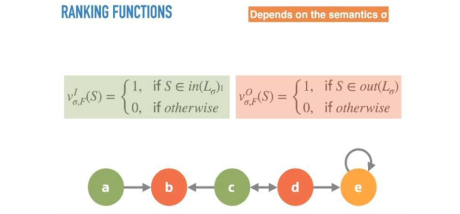
\includegraphics[width=13cm, keepaspectratio]{img/Cap8/ordinamento-quantitativo.png}
\end{figure}

\begin{itemize}
    \item La funzione verde assegna agli argomenti il valore 1 se sono
          argomenti IN che sono accettati da qualche semantica $\sigma$, oppure 0.
          Se calcolo il valore per l'insieme a, c questo darà 1 perché l'insieme è
          IN.
    \item La funzione rossa invece di guardare gli argomenti che sono IN e
          dargli punteggio 1, guarda quelli OUT e gli da punteggio 1 in maniera
          negativa.
\end{itemize}
Quindi se la funzione $V^I$ da punteggio 1 significa che sono una buona
estensione, se la funzione $V^O$ da punteggio 1 allora sono una cattiva
estensione. Adesso quindi siamo arrivati al punto di avere per ogni insieme
di argomenti un valore che è 0 o 1 in base alla funzione per gli IN o per
gli OUT e quindi possiamo generare un ordinamento.
\paragraph{Ordinamento degli argomenti in base al valore}
\begin{figure}[htp]
    \centering
    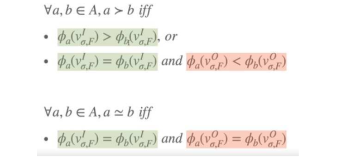
\includegraphics[width=10cm, keepaspectratio]{img/Cap8/ordinamento-valore.png}
\end{figure}
\textbf{Il primo punto si traduce in:}
\\L'argomento a è \textbf{migliore} dell' argomento b se e soltanto se:
\begin{itemize}
    \item Lo Shapely value di a rispetto agli argomenti IN è maggiore dello
          Shapely value di b sempre rispetto agli argomenti IN.
    \item Oppure se il valore è uguale (quindi non mi basta andare a controllare
          solamente gli IN), a deve avere anche uno Shapely value per gli OUT minore
          di quello di b.
\end{itemize}
\begin{center}
    \textbf{Il secondo punto è l'indifferenza}
\end{center}
Scegliere prima a o b è indifferente se e soltanto se:
\begin{itemize}
    \item Lo Shapely value per gli IN di a è esattamente uguale allo Shapely
          value per gli IN di b e stessa cosa per il valore di OUT.
\end{itemize}
